\chapter{文件系统}

Unix系统有一个基本设计哲学——“一切皆是文件”,它指的是系统中的一切都可以用文件的方式访问、
管理,即使它不是文件。比如硬件设备、进程等等,都可以抽象成文件,使用统一的用户接口。

\section{系统设计}

NimlothOS借鉴这一设计哲学,实现了一个简单的分层文件系统,从系统调用接口到底层块设备驱动。
文件系统支持文件创建、读写、删除等基本操作,以及管道通信和标准输入输出重定向功能。
它含有以下内容:

\begin{itemize}
    \item \textbf{系统调用接口}:提供read、write、open、close等标准POSIX接口
    \item \textbf{OSInode}:操作系统级文件抽象,管理文件偏移量和权限
    \item \textbf{Inode文件管理器}:文件系统抽象层,提供文件和目录操作
    \item \textbf{磁盘块管理器}:负责磁盘数据结构的管理
    \item \textbf{磁盘布局}:定义SuperBlock、DiskInode等磁盘数据结构
    \item \textbf{位图管理}:管理inode和数据块的分配与回收
    \item \textbf{块缓存}:提供高效的磁盘块缓存机制
    \item \textbf{块设备抽象}:定义统一的块设备接口
    \item \textbf{硬件驱动}:具体的块设备驱动实现
\end{itemize}

\begin{figure}[htbp]
    \centering
    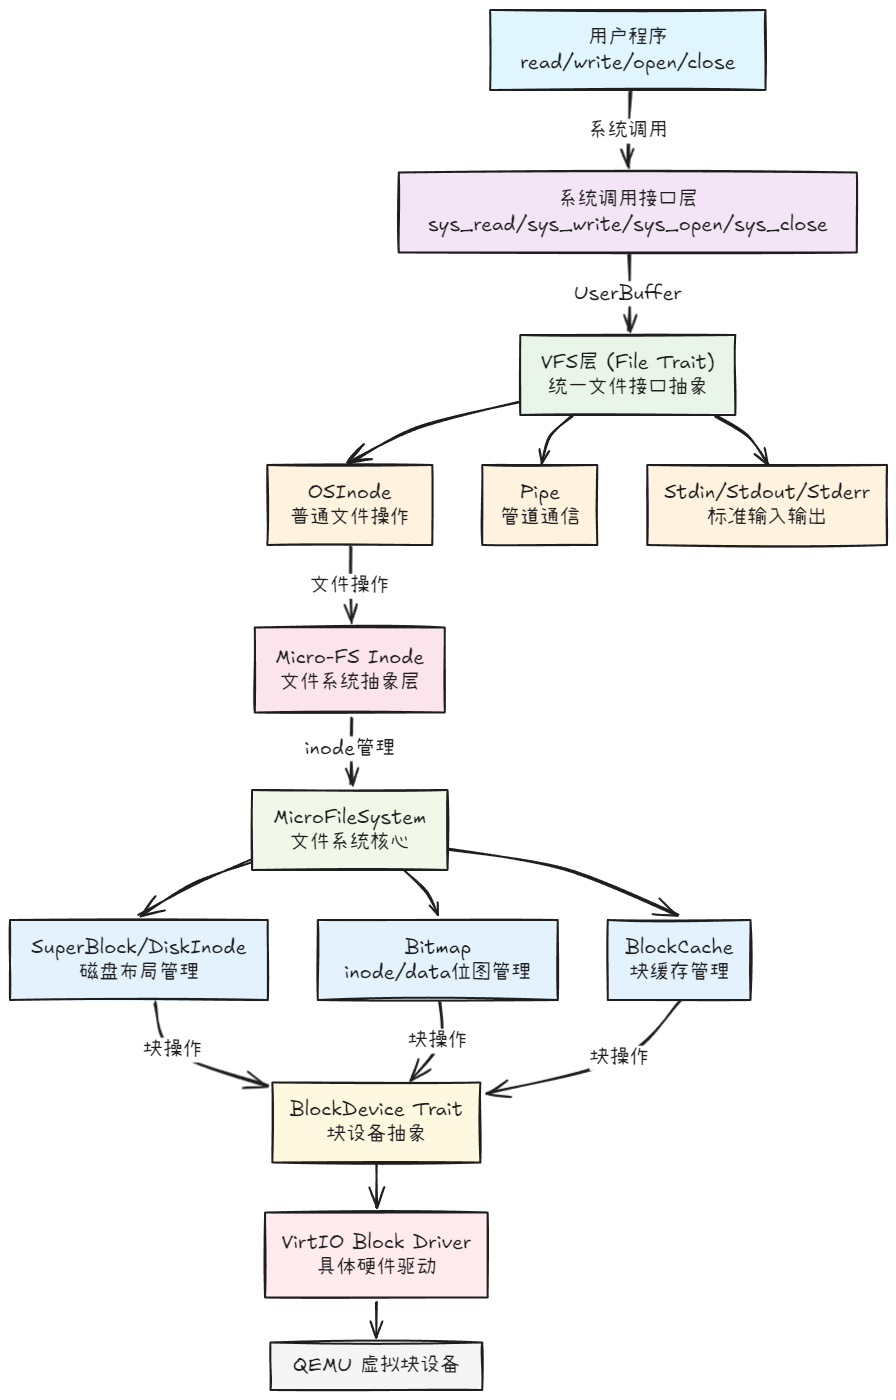
\includegraphics[width=0.8\textwidth]{../image/文件系统.png}
    \caption{文件系统分层架构}
    \label{fig:filesystem-arch}
\end{figure}

\clearpage

\noindent
\rule{0.4\textwidth}{0.4pt}
\hfill
\text{以下为实现介绍}
\hfill
\rule{0.4\textwidth}{0.4pt}

\section{块缓存}

块缓存是文件系统的性能优化核心,它通过在内存中缓存频繁访问的磁盘块来减少实际的磁盘I/O操作。NimlothOS的块缓存采用LRU(最近最少使用)策略,能够有效提高文件系统的读写性能。

\begin{lstlisting}[language=Rust]
pub struct BlockCache {
    cache: [u8; BLOCK_SZ],
    block_id: usize,
    block_device: Arc<dyn BlockDevice>,
    modified: bool,
}

impl BlockCache {
    pub fn sync(&mut self) {
        if self.modified {
            self.modified = false;
            self.block_device.write_block(self.block_id, &self.cache);
        }
    }
}
\end{lstlisting}

每个\texttt{BlockCache}实例代表一个被缓存的磁盘块,包含了512字节的数据缓存、对应的块号、块设备引用以及修改标记。
当缓存中的数据被修改时,系统会设置\texttt{modified}标记,并在适当的时机通过\texttt{sync}方法将数据写回磁盘。
通过这样的延迟写入,可以有效减少磁盘写入次数。

块缓存管理器负责协调多个块缓存的分配和回收,它维护一个固定大小的缓存池,当缓存满时会根据LRU策略替换最久未使用的块。
系统还提供了\texttt{block\_cache\_sync\_all}函数来强制同步所有被修改的缓存到磁盘。

\section{磁盘布局及其数据结构}

\subsection{磁盘布局}

磁盘按照块编号从小到大,可以分成五个区域。第一块是超级块,它用于存放魔数进行文件系统合法性检查,
并存放剩下几个块的位置;第二个区域是索引节点位图,用于记录索引节点是否被使用;第三个区域是索引节点,
用于记录文件的元数据;第四个区域是数据块位图,用于记录数据块是否被使用;第五个区域是数据块,
用于存放文件数据和目录项数据。

\begin{figure}[htbp]
    \centering
    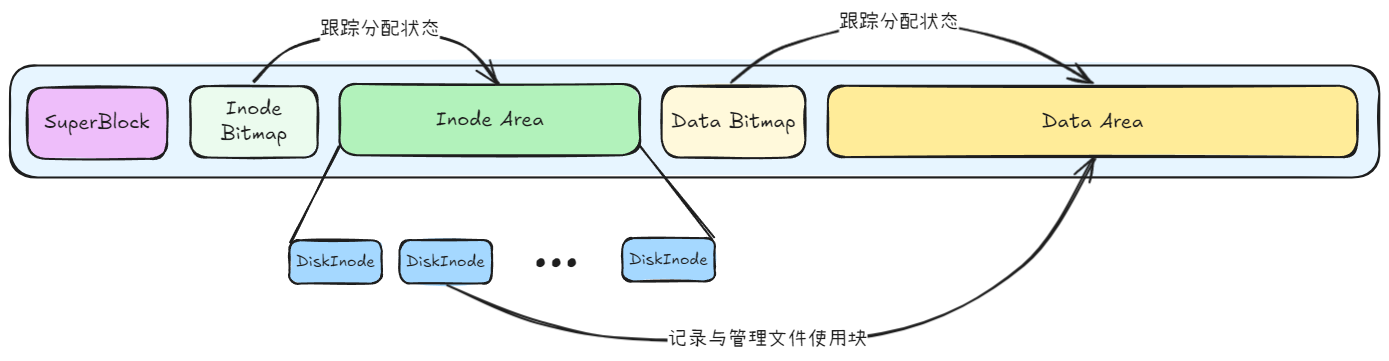
\includegraphics[width=0.8\textwidth]{../image/文件系统磁盘结构.png}
    \caption{磁盘布局}
    \label{fig:disk-layout}
\end{figure}

\subsection{超级块}

超级块存储着整个文件系统的全局信息。它位于磁盘的第0块,包含了文件系统的基本参数和各个区域的布局信息。

\begin{lstlisting}[language=Rust]
#[repr(C)]
pub struct SuperBlock {
    magic: u32,
    pub total_blocks: u32,
    pub inode_bitmap_blocks: u32,
    pub inode_area_blocks: u32,
    pub data_bitmap_blocks: u32,
    pub data_area_blocks: u32,
}

impl SuperBlock {
    pub fn initialize(&mut self, total_blocks: u32, inode_bitmap_blocks: u32,
                     inode_area_blocks: u32, data_bitmap_blocks: u32,
                     data_area_blocks: u32) {
        *self = Self {
            magic: MFS_MAGIC,
            total_blocks, inode_bitmap_blocks, inode_area_blocks,
            data_bitmap_blocks, data_area_blocks,
        }
    }

    pub fn valid(&self) -> bool {
        self.magic == MFS_MAGIC
    }
}
\end{lstlisting}

它通过魔数\texttt{MFS\_MAGIC}来验证文件系统的合法性。其余字段负责记录各个区域占用的块数,当系统启动时,会首先读取超级块来获取整个文件系统的布局信息。

\subsection{位图}

磁盘上有两块位图区域,一块是索引节点位图,一块是数据块位图。位图采用位操作来管理资源的分配状态,每个位对应一个资源单元的使用情况。

\begin{lstlisting}[language=Rust]
pub struct Bitmap {
    start_block_id: usize,
    blocks: usize,
}

impl Bitmap {
    pub fn alloc(&self, block_device: &Arc<dyn BlockDevice>) -> Option<usize> {
        for block_id in 0..self.blocks {
            let pos = block_cache(block_id + self.start_block_id as usize,
                                 Arc::clone(block_device))
                .lock()
                .modify(0, |bitmap_block: &mut BitmapBlock| {
                    if let Some((bits64_pos, inner_pos)) = bitmap_block
                        .iter().enumerate()
                        .find(|(_, bits64)| **bits64 != u64::MAX)
                        .map(|(bits64_pos, bits64)| 
                             (bits64_pos, bits64.trailing_ones() as usize))
                    {
                        bitmap_block[bits64_pos] |= 1u64 << inner_pos;
                        Some(block_id * BLOCK_BITS + bits64_pos * 64 + inner_pos)
                    } else { None }
                });
            if pos.is_some() { return pos; }
        }
        None
    }
}
\end{lstlisting}

位图的实现利用了64位整数的位操作特性,每个\texttt{u64}可以表示64个资源单元的状态。分配算法采用首次适应策略,
从第一个位图块开始查找第一个可用的位。通过\texttt{trailing\_ones}方法能够快速定位到第一个0位。

\subsection{索引节点}

索引节点(inode)是文件系统中每个文件和目录的控制结构,它包含了文件的所有元数据信息以及数据块的索引信息。

\begin{lstlisting}[language=Rust]
#[repr(C)]
pub struct DiskInode {
    pub size: u32,
    pub direct: [u32; INODE_DIRECT_COUNT],
    pub indirect1: u32,
    pub indirect2: u32,
    pub indirect3: u32,
    type_: DiskInodeType,
}

impl DiskInode {
    pub fn block_id(&self, inner_id: u32, 
                   block_device: &Arc<dyn BlockDevice>) -> u32 {
        let inner_id = inner_id as usize;
        if inner_id < INODE_DIRECT_COUNT {
            self.direct[inner_id]
        } else if inner_id < INDIRECT1_BOUND {
            block_cache(self.indirect1 as usize, Arc::clone(block_device))
                .lock()
                .read(0, |indirect_block: &IndirectBlock| {
                    indirect_block[inner_id - INODE_DIRECT_COUNT]
                })
        } else {
            // 处理二级和三级间接块的情况...
        }
    }
}
\end{lstlisting}

inode设计采用了多级索引结构,包含27个直接块索引、一个一级间接块索引、一个二级间接块索引和一个三级间接块索引。这样既能通过直接块高效处理小文件,
又能通过间接块支持大文件。直接块能够快速访问文件的前13.5KB数据,而间接块结构则能够支持最大约1GB的文件大小。

\subsection{数据块}

数据块是文件系统中实际存储文件内容和目录项的区域。每个数据块大小为512字节。数据块的读写操作考虑了跨块访问的情况,
当文件读写操作跨越多个块时,系统会自动处理块边界,确保数据的连续性和完整性。这样使得上层应用可以透明地进行任意大小和位置的文件读写操作。

\section{磁盘块管理器}

磁盘块管理器(BlockManager)是Micro File System的核心组件,它负责管理整个文件系统的状态和操作,包括文件系统的创建、打开、资源分配和回收等功能。

\begin{lstlisting}[language=Rust]
pub struct BlockManager {
    pub block_device: Arc<dyn BlockDevice>,
    pub inode_bitmap: Bitmap,
    pub data_bitmap: Bitmap,
    inode_area_start_block: u32,
    data_area_start_block: u32,
}

impl BlockManager {
    pub fn create(block_device: Arc<dyn BlockDevice>, total_blocks: u32,
                 inode_bitmap_blocks: u32) -> Arc<Mutex<Self>> {
        let inode_bitmap = Bitmap::new(1, inode_bitmap_blocks as usize);
        let inode_num = inode_bitmap.maximum();
        let inode_area_blocks = 
            ((inode_num * core::mem::size_of::<DiskInode>() + BLOCK_SZ - 1) 
             / BLOCK_SZ) as u32;
        
        // 创建文件系统实例并初始化所有数据结构
        let mut mfs = Self {
            block_device: Arc::clone(&block_device),
            inode_bitmap,
            data_bitmap: Bitmap::new((1 + inode_total_blocks) as usize,
                                   data_bitmap_blocks as usize),
            inode_area_start_block: 1 + inode_bitmap_blocks,
            data_area_start_block: 1 + inode_total_blocks + data_bitmap_blocks,
        };
        
        // 初始化根目录
        assert_eq!(mfs.alloc_inode(), 0);
        Arc::new(Mutex::new(mfs))
    }
}
\end{lstlisting}

磁盘块管理器的创建过程如上。它首先根据指定的参数计算各个区域的大小和位置,然后清空所有数据块,创建超级块,最后初始化根目录inode。
这个过程确保了文件系统从一开始就处于一致和可用的状态。根目录的inode号固定为0,使得系统能够快速定位到文件系统的入口点。

磁盘块管理器还提供了资源分配和回收的功能,包括inode分配、数据块分配以及对应的释放操作。这些操作都通过位图来管理,
确保资源分配的高效性和一致性。

\section{Inode文件管理器}

Inode文件管理器提供了文件系统的抽象接口,它封装了底层磁盘inode的复杂性,为上层提供了简洁易用的文件操作API。

\begin{lstlisting}[language=Rust]
pub struct Inode {
    block_id: usize,
    block_offset: usize,
    fs: Arc<Mutex<BlockManager>>,
    block_device: Arc<dyn BlockDevice>,
}

impl Inode {
    pub fn find(&self, path: &str) -> Option<Arc<Inode>> {
        let fs = self.fs.lock();
        let mut block_id = self.block_id as u32;
        let mut block_offset = self.block_offset;
        for name in path.split('/').filter(|s| !s.is_empty()) {
            let inode_id = block_cache(block_id as usize, self.block_device.clone())
                .lock()
                .read(block_offset, |disk_inode: &DiskInode| {
                    if disk_inode.file() { return None; }
                    self.find_inode_id(name, disk_inode)
                });
            if inode_id.is_none() { return None; }
            (block_id, block_offset) = fs.disk_inode_pos(inode_id.unwrap());
        }
        Some(Arc::new(Self::new(block_id, block_offset, 
                               self.fs.clone(), self.block_device.clone())))
    }

    pub fn create(&self, name: &str) -> Option<Arc<Inode>> {
        self.create_inode(name, DiskInodeType::File)
    }
}
\end{lstlisting}

Inode文件管理器将复杂的磁盘操作隐藏在简洁的接口后面。\texttt{find}方法支持路径查找,能够从当前目录开始逐级查找到目标文件或目录。文件创建操作通过\texttt{create}方法实现,它会在当前目录中分配新的inode并添加相应的目录项。

这一层的设计使得文件系统具有了面向对象的特性,每个Inode对象都代表一个具体的文件或目录,用户可以通过这些对象进行各种文件操作,如读写、创建子文件、列出目录内容等。

\section{OSInode}

OSInode是操作系统级别的文件抽象层,它在Inode文件管理器的基础上增加了进程相关的文件操作语义,如文件偏移量管理和权限控制。

\begin{lstlisting}[language=Rust]
pub struct OSInode {
    readable: bool,
    writable: bool,
    inner: UPSafeCell<OSInodeInner>,
}

pub struct OSInodeInner {
    offset: usize,
    inode: Arc<Inode>,
}

impl File for OSInode {
    fn read(&self, mut buf: UserBuffer) -> usize {
        let mut inner = self.inner.exclusive_access();
        let mut total_read_size = 0usize;
        for slice in buf.buffers.iter_mut() {
            let read_size = inner.inode.read_at(inner.offset, *slice);
            if read_size == 0 { break; }
            inner.offset += read_size;
            total_read_size += read_size;
        }
        total_read_size
    }

    fn write(&self, buf: UserBuffer) -> usize {
        let mut inner = self.inner.exclusive_access();
        let mut total_write_size = 0usize;
        for slice in buf.buffers.iter() {
            let write_size = inner.inode.write_at(inner.offset, *slice);
            assert_eq!(write_size, slice.len());
            inner.offset += write_size;
            total_write_size += write_size;
        }
        total_write_size
    }
}
\end{lstlisting}

OSInode为文件操作引入了进程级别的状态管理。每个OSInode实例都维护着独立的文件偏移量,这使得不同进程或同一进程的不同文件描述符可以独立地访问同一个文件。读写权限控制确保了文件访问的安全性,防止了不当的文件操作。

通过实现File trait,OSInode与系统VFS层的集成,文件也可以像其他系统资源一样被统一管理。这也为进程文件描述符表的实现提供了基础,每个文件描述符实际上就是一个OSInode实例的引用。

\section{基于文件的管道机制}

管道机制是进程间通信的重要手段,NimlothOS实现了基于文件接口的管道,使得管道可以像普通文件一样被操作。

\begin{lstlisting}[language=Rust]
pub struct Pipe {
    readable: bool,
    writable: bool,
    buffer: Arc<UPSafeCell<PipeRingBuffer>>,
}

pub struct PipeRingBuffer {
    arr: [u8; RING_BUFFER_SIZE],
    head: usize,
    tail: usize,
    status: RingBufferStatus,
    write_end: Option<Weak<Pipe>>,
}

impl File for Pipe {
    fn read(&self, buf: UserBuffer) -> usize {
        assert!(self.readable);
        let mut already_read = 0usize;
        loop {
            let mut ring_buffer = self.buffer.exclusive_access();
            let loop_read = ring_buffer.available_read();
            if loop_read == 0 {
                if ring_buffer.all_write_ends_closed() {
                    return already_read;
                }
                drop(ring_buffer);
                suspend_current_and_run_next();
                continue;
            }
            // 从环形缓冲区读取数据...
        }
    }
}

pub fn make_pipe() -> (Arc<Pipe>, Arc<Pipe>) {
    let buffer = Arc::new(unsafe { UPSafeCell::new(PipeRingBuffer::new()) });
    let read_end = Arc::new(Pipe::read_end_with_buffer(buffer.clone()));
    let write_end = Arc::new(Pipe::write_end_with_buffer(buffer.clone()));
    (read_end, write_end)
}
\end{lstlisting}

管道的实现基于环形缓冲区。读端在缓冲区为空时会阻塞等待,写端在缓冲区满时也会阻塞等待,这种阻塞机制通过进程调度器实现,能够有效协调进程间的数据传输。

管道的生命周期管理通过弱引用实现,当所有写端关闭且缓冲区为空时,读端会收到EOF信号。这种设计确保了管道在进程结束或文件描述符关闭时能够正确清理资源。

\section{标准输入输出}

标准输入输出是每个进程必备的基础设施,NimlothOS为每个进程提供了三个标准文件描述符:stdin、stdout和stderr。

\begin{lstlisting}[language=Rust]
pub struct Stdin;
pub struct Stdout;
pub struct Stderr;

impl File for Stdin {
    fn read(&self, mut user_buf: UserBuffer) -> usize {
        assert_eq!(user_buf.len(), 1);
        let mut c: usize;
        loop {
            c = console_getchar();
            if c == 0 {
                suspend_current_and_run_next();
                continue;
            } else { break; }
        }
        let ch = c as u8;
        unsafe {
            user_buf.buffers[0].as_mut_ptr().write_volatile(ch);
        }
        1
    }
}

impl File for Stdout {
    fn write(&self, user_buf: UserBuffer) -> usize {
        for buffer in user_buf.buffers.iter() {
            print!("{}", core::str::from_utf8(*buffer).unwrap());
        }
        user_buf.len()
    }
}
\end{lstlisting}

标准输入的实现采用了阻塞式读取策略,当没有输入数据时会主动让出CPU。标准输出和标准错误都直接输出到控制台,支持UTF-8编码的文本处理。

这些标准设备同样实现了File trait,因此可以与文件系统的其他组件无缝集成。进程在创建时会自动分配这三个标准文件描述符,为应用程序提供统一的I/O接口。

\section{标准I/O重定向}

基于统一的File trait接口,NimlothOS能够轻松实现标准I/O重定向功能。进程可以将标准输入重定向到文件或管道,将标准输出重定向到文件、管道或其他设备。
这都依赖于文件描述符表。由于所有的I/O对象都实现了相同的File trait,因此可以在运行时动态替换文件描述符表中的对象,从而实现各种形式的I/O重定向。
这也为shell命令管道、文件重定向等功能提供了支持。
